\documentclass{llncs}
%
\usepackage{cite}
\usepackage{llncsdoc}
\usepackage[ngerman,colorlinks=true]{hyperref}
\usepackage[ngerman,english]{babel}
\usepackage[utf8]{inputenc}
\bibliographystyle{splncs}

\usepackage{libertine}
\usepackage{pifont}
\usepackage{microtype}
\usepackage{textcomp}
\usepackage{graphicx}

\begin{document}

\title{GSem Ausarbeitung: Überblick EAM}
\subtitle{Chancen für agiles Enterprise Architecture Management durch Aufstrebende Technologische Paradigmen wie Continuous Delivery, DevOps und Microservices}
\author{Daniel Kirchner}
\institute{HAW Hamburg, 20099 Hamburg, Germany}
\maketitle
%
\begin{abstract}
Es wird eine Auswahl von neuen technologischen Paradigmen betrachtet, bei denen zur Zeit wachsendes Interesse und erste positive Erfahrungen in dem Betrieb und der Entwicklung von Software beobachtet werden.
Aus diesen wird versucht einen allgemeinen Trend zu erkennen und es werden Verknüpfungspunkte zu klassischen Frameworks aus dem Enterprise Architecture Management und der IT Governance vorgeschlagen.
Die Ergebnisse werden unter den Gesichtspunkten \textit{lean}, \textit{agile} und \textit{collaborative} diskutiert.
\end{abstract}
%
\section{Motivation}
%
Informationstechnologie hat sich als lebenswichtiger Aspekt in allen Bereichen großer Unternehmen längst etabliert. Selbst in Unternehmen, deren Kerngeschäft nicht in der Informationstechnologie selbst liegt, werden Geschäftsprozesse - bewusst oder unbewusst - in der Architektur und dem Datenaustausch der betriebenen Systeme abgebildet.\\

Produkte selbst, ihre Entwicklung und ihr Verkauf, der Kontakt zu Kunden und Lieferanten, Supply-Chain, die Verwaltung der Mitarbeiter und Prozesse aus Controlling und Finanzwesen sind nur wenige Beispiele aus einer sehr langen Liste von Bereichen, die inzwischen von Softwareprodukten mehrerer Generationen unterstützt und teilweise automatisiert werden.\\

Dabei werden nicht nur Daten erzeugt, verteilt und konsumiert, sondern zunehmend wird auch eine intelligente Verarbeitung der eigenen Daten automatisiert. Dabei werden z.B. Aufgaben aus der Planung, Anomalienerkennung und der Vorhersage automatisiert, die vorher von Menschen übernommen wurde. Dabei entstehen wiederum neue Anforderungen an eine systematische Datenerfassung von neuen - und insbesondere auch von bestehenden - Systemen.\\

Das Problem, die IT-Landschaft eines Unternehmens ständig neuen Bedürfnissen anzupassen und dabei einen möglichst
schlanken und stabilen Betrieb sicherzustellen, ist seit Jahrzehnten Gegenstand von wissenschaftlicher und industrieller Forschung.\\

In den letzten Jahren haben Techniken aus der Softwareentwicklung mit pragmatischen Ansätzen, kurzen Feedbackzyklen und kleinen Teams gute Resultate in der Umsetzung komplexer Softwareprojekte erzielt und die Aufmerksamkeit des \textit{Enterprise Architecture Managements} erregt\cite{buc:mat}.\\

In diesem Aufsatz werden konkrete Möglichkeiten erläutert aufstrebende technologische Paradigmen in eine \textit{Enterprise Architecture} zu integrieren und Verknüpfungen zum \textit{Enterprise Architecture Management} erläutert.

%
\section{Grundlagen des Enterprise Architecture Managements}
\subsection{Definition und Scope}
Nach \cite{ben} ergeben sich folgende Arbeitsdefinitionen von \textit{Enterprise Architecture} und \textit{Enterprise Architecture Management}:\\

\textbf{\textit{Enterprise Architecture (EA)}} ist eine Repräsentation der Struktur und des Verhaltens der IT-Landschaft eines Unternehmens mit Bezug auf das geschäftliche Umfeld. Dabei stellt sie die momentane und die zukünftige Nutzung von IT im Unternehmen dar und liefert einen Plan zur Erreichung eines zukünftigen Zustands. Dabei bietet sie
%
\begin{itemize}
	\item Einsichten in die IT-Nutzung aus Sicht des Geschäftsbetriebs
	\item eine Vision für die zukünftige Nutzung von IT im Geschäftsbetrieb
	\item einen Plan für schrittweise Evolution hin zu einem zukünftigen Zustand
\end{itemize}

%
\textbf{\textit{Enterprise Architecture Management (EAM)}} ist ein strukturierter Ansatz um \textit{EA} zu erzeugen, zu verwalten und anzuwenden um die IT-Nutzung am Geschäftsbetrieb auszurichten. Dabei übersetzt \textit{EAM} die geschäftliche Vision in konkrete Unternehmungen und begleitet das Unternehmen vom jeweils aktuellen EA-Zustand bis zu einem Zielzustand.
 
\subsection{Tools und Frameworks}
Um einen gemeinsamen Wortschatz der Beteiligten des \textit{EAM} zu schaffen, aber auch um eine Sammlung von bewährten Richtlinien, Prozessen und Dokumenten verfügbar zu machen wurden verschiedenste \textit{EAM}-Frameworks entwickelt.\\

Zu den wichtigsten (siehe \cite{ben}) Frameworks gehören das Zachman Framework\footnote{https://www.zachman.com/about-the-zachman-framework, abgerufen am 03.06.2015}, das Open Group Architecture Framework (TOGAF)\footnote{https://www.opengroup.org/togaf/, abgerufen am 03.06.2015} und die Gartner Methodologies\footnote{http://www.gartner.com/technology/research/methodologies/methodology.jsp, abgerufen am 03.06.2015}.
%
\section{Übersicht der betrachteten Technologischen Paradigmen}
%
\subsection{Continuous Delivery}
\textbf{\textit{Continous Delivery}} ist eine Erweiterung von \textit{Continous Integration}, die als Methodik der Softwareentwicklung bereits erfolgreich in Unternehmen etabliert ist (\cite{fit:sto}).

Wesentliches Ziel ist eine schnelle Rückmeldung für eingepflegten Code durch möglichst unmittelbare Auslieferung der Änderung bis in das laufende System zu erreichen. Dabei wird eine Automatisierungslinie (\textit{continuous delivery pipeline}) geschaffen, die Build, Tests und Deployment des geänderten produktiven Systems soweit automatisiert, dass möglichst schnell Werte (im Sinne von produktiv eingesetzten Features) geschaffen werden (Vgl \cite{wolff}).
%
\subsection{Microservices}
Mit dem \textit{Microservices}-Architekturparadigma wird eine Art der Entkopplung von Softwarekomponenten beschrieben, bei denen die Komponenten in eigenen betriebssystemartigen Umgebungen existieren.\\

Durch die Weiterentwicklung von Technologien zur Erzeugung und Verwaltung solcher Anwendungscontainer, wie \textit{Docker}\footnote{https://www.docker.com/, abgerufen am 03.06.2015} und \textit{Rocket}\footnote{https://coreos.com/blog/rocket/, abgerufen am 03.06.2015}, ist es möglich die automatische Erzeugung solcher Container - und damit das Deployment von Softwarekomponenten - drastisch zu vereinfachten. Dieses ist ein wesentliches Element bei dem Übergang von \textit{Continuous Delivery} zu \textit{Continuous Deployment} (\cite{wolff}).\\

Zudem ist es möglich mit dieser Art des Anwendungsbetriebes Architekturen umzusetzen, die den Wartungsaufwand und die horizontale Skalierbarkeit von Anwendungen deutlich verbessern (\cite{tof:bru}).

\subsection{DevOps}
\textit{DevOps} bezeichnet ein Paradigma der engen Verknüpfung zwischen Verantwortung für die Entwicklung und dem produktiven Betrieb von Softwarekomponenten.\\
Bei der Umsetzung einer \textit{Continuous Delivery Pipeline} ist für die Produktionstauglichkeit der Software neben den üblichen Tests auf Korrektheit der Implementation besonders die Performance im realen Betrieb ein kritischer Punkt (\cite{wal:ehm}).

\section{Vorschlag zur integrierten Umsetzung der Paradigmen auf Unternehmensebene}
Setzt man die betrachteten technologischen Paradigmen in einer idealisierten Architektur um, könnte sich etwa ein Modell wie in Abb~\ref{fig:model} dargestellt ergeben.\\

Es wird eine vertikale Aufteilung der IT-Landschaft vorgenommen, die fast ausschließlich an den geschäftlichen Kategorien orientiert ist (Ausnahme ist der Betrieb von technischer Infrastruktur). Dabei werden über \textit{Continuous Delivery} möglichst kurze Feedbackwege über den gesamten Stack von den geschäftlichen Anforderungen bis zum Betrieb und der Performance einzelner Dienste im Backend geschaffen.\\

\begin{figure}[ht!]
	\centering
  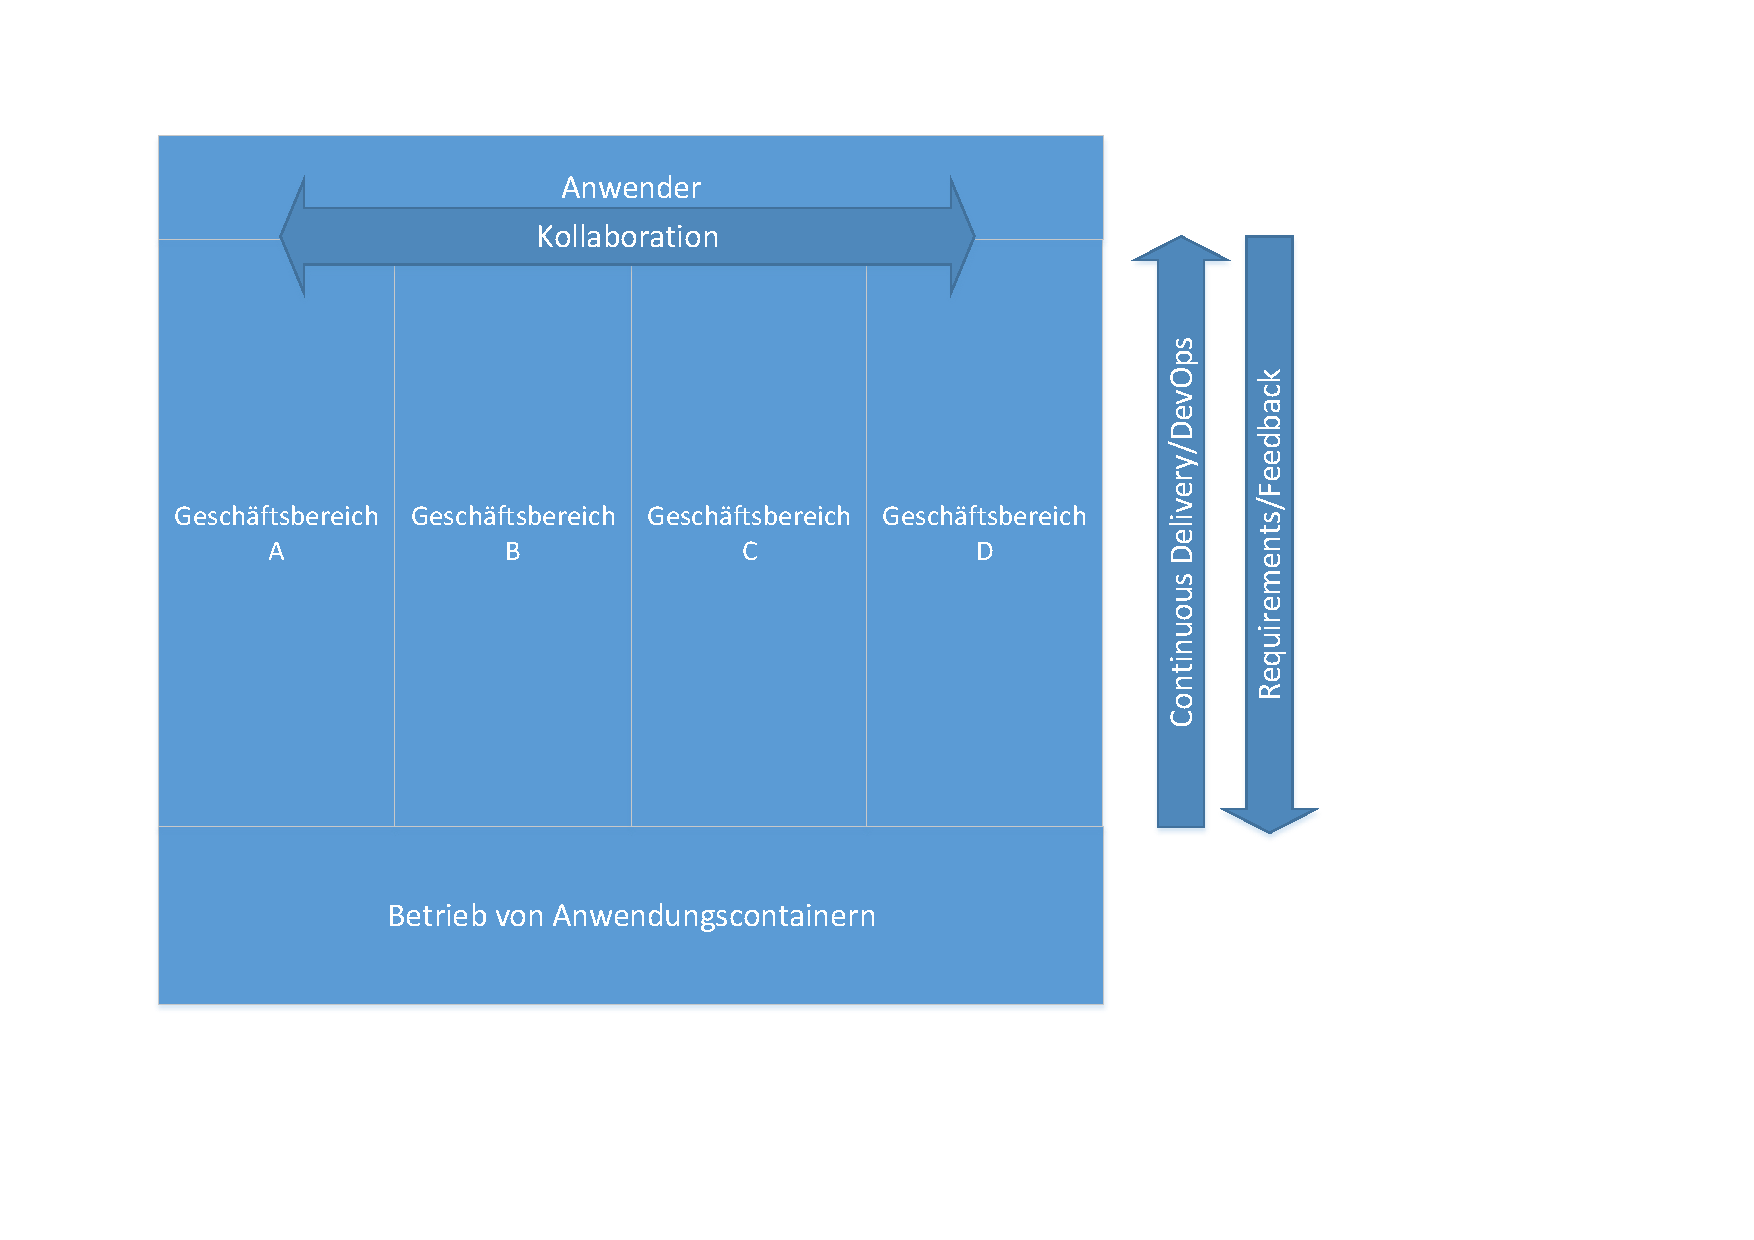
\includegraphics[scale=0.5]{simple_diagram.pdf}
	\caption{Naive Sicht auf eine Continuous-Delivery-zentrierte Unternehmensarchitektur}
	\label{fig:model}
\end{figure}

Aus dieser Betrachtung ergibt sich in erster Näherung eine mögliche Architektur für IT-Landschaften von Unternehmen, die sich den agilen Werten\footnote{http://agilemanifesto.org/, abgerufen am 03.06.2015} annähern könnte:

\begin{itemize}
\item Individuals and interactions over processes and tools
\item Working software over comprehensive documentation
\item Customer collaboration over contract negotiation
\item Responding to change over following a plan
\end{itemize}

\section{Zusammenfassung und Ausblick}
Es wurde erläutert, dass aus einer sehr oberflächlichen Betrachtung heraus durchaus die Möglichkeit bestehen könnte durch konkrete Einflechtung der genannten technologischen Paradigmen einen erhöhten Reifegrad (\textit{Maturity Level}) bezüglich Agilität und Kollaboration durch und innerhalb von Unternehmens-IT zu erreichen.\\

Es stellen sich jedoch viele offene Fragen, die in weiterer Literaturrecherche und auch im Experiment behandelt werden müssten, beispielsweise:
\begin{itemize}
	\item Wie wird eine sinnvolle Aufteilung in Geschäftsbereiche gemessen?
	\item Welche Metriken existieren?
	\item Wie groß ist der Einfluss von Duplikation von Komponenten?
	\item Wie geht das vorgeschlagene Modell mit Korrosion seiner Struktur um?
	\item Welche Artefakte von üblichen EAM-Frameworks lassen sich noch anwenden, welche müssen angepasst werden?
	\item Wie könnte eine Transition von einer bestehenden Architektur aussehen?
	\item Welchen Einfluss hat das Modell auf Sicherheits- und Verfügbarkeitsrisiken?
\end{itemize}

Das \textit{HAW Labor für Anwendungsintegration} ist dabei ein Bereich, der für die Untersuchung vieler dieser Fragen einen akademisch geschlossenes und dennoch realitätsnahes Umfeld bietet.\\

Ein konkreter Einstieg könnte sein, im Rahmen eines Grundprojektes die technischen Vorraussetzungen für eine \textit{Continuous Delivery Pipeline} in einem technisch und geschäftlich heterogenen Umfeld zu schaffen.\\

Durch zweimal jährlich wechselnde Studentengruppen (in der Rolle der Softwareentwickler) und die Abwesenheit des Risikos geschäftsvernichtender, katastrophaler Systemausfälle sind dann die Rahmenbedingungen für weiterführende Untersuchungen und Experimente gegeben.

\cite{SeojinKim:2008:ACI:1642931.1642990}
\cite{clar:eke}

%%%%%%%%%%%%

\begin{thebibliography}{1}
\bibitem {clar:eke}
Clarke, F., Ekeland, I.:
Nonlinear oscillations and boundary-value problems for
Hamiltonian systems.
Arch. Rat. Mech. Anal. 78, 315--333 (1982)

\bibitem {kim:park}
Kim, S., Park, S.:
Automated Continuous Integration of Component-Based Software: An Industrial Experience
ASE '08 Proceedings of the 2008 23rd IEEE/ACM International Conference on Automated Software Engineering
Pages 423-426

\bibitem {ben}
Bente, S.:
Collaborative Enterprise Architecture
2011 Morgan Kaufmann Publ.

\bibitem {hay:skat}
Haynes, S., Skattebo, A.:
Collaborative architecture design and evaluation
DIS '06 Proceedings of the 6th conference on Designing Interactive systems
Pages 219-228

\bibitem {buc:mat}
Buckl, S., Matthes, F.:
Towards an Agile Design of the Enterprise Architecture Management Function
2011 15th IEEE International Enterprise Distributed Object Computing Conference Workshops
Pages 322-329

\bibitem {fit:sto}
Fitzgerald, F., Stol, K.-J.:
Continuous software engineering and beyond: trends and challenges
RCoSE 2014 Proceedings of the 1st International Workshop on Rapid Continuous Software Engineering
Pages 1-9

\bibitem {wolff}
Wolf, D.:
Continuous Delivery: Der pragmatische Einstieg
2014 dpunkt.verlag GmbH

\bibitem {tof:bru}
Toffetti, G., Brunner, S.:
An architecture for self-managing microservices
AIMC '15 Proceedings of the 1st International Workshop on Automated Incident Management in Cloud
Pages 19-24

\bibitem {wal:ehm}
Waller, J., Ehmke, N.:
Including Performance Benchmarks into Continuous Integration to Enable DevOps
ACM SIGSOFT Software Engineering Notes archive
Volume 40 Issue 2, March 2015 
Pages 1-4 
%
\end{thebibliography}

\end{document}